\section{Conceitos básicos}

A trigonometria teve origem com o estudo das relações entre as medidas dos lados e dos ângulos de um triângulo retângulo. Posteriormente, o estudo foi estendido para outros “ambientes”, como a circunferência trigonométrica. Com isso, as funções trigonométricas foram amplamente estudadas: seno, cosseno, tangente, cossecante, secante e cotangente. Este material aborda os conceitos básicos de trigonometria, as funções trigonométricas e suas relações e transformações.

Hoje em dia a trigonometria não se limita estudar somente os triângulos. Encontramos aplicações da trigonometria em eletricidade, mecânica, acústica, música, engenharias e muitos outros campos de atividades.

\subsection{Trigonometria no triângulo retângulo}

Se um triângulo possuir um de seus ângulos internos reto, então ele é chamado de triângulo retângulo. Na Figura \ref{fig:01}, o triângulo ABC ($\Delta ABC$) é um triângulo retângulo com ângulo reto $\hat{A}$ e ângulos agudos $\hat{B}$ e $\hat{C}$.

    \begin{figure}[h]
        \centering
        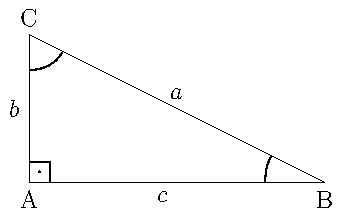
\includegraphics[scale=0.8]{Imagens/fig01.pdf}
        \caption{triângulo retângulo ($\Delta ABC$)}
        \label{fig:01}
    \end{figure}

    \begin{itemize}
        \item O lado BC do $\Delta ABC$ é chamado de hipotenusa e mede a
        \item 	O lado AC do $\Delta ABC$ é chamado de cateto oposto ao ângulo $\hat{B}$ mede b. Este mesmo lado é chamado de cateto adjacente ao ângulo $\hat{C}$
        \item O lado AB do $\Delta ABC$ é chamado de cateto oposto ao ângulo $\hat{C}$ e mede c. Este mesmo lado é chamado de cateto adjacente ao ângulo $\hat{B}$.
    \end{itemize}

Tem-se, por definição, que:

\begin{tcolorbox}[colback=white,colframe=minha_cor,coltitle=black,title=Definição de seno] 
\begin{equation}
    \sen \hat{B} = \df{\text{medida do cateto oposto à } \hat{B}}{\text{medida da hipotenusa}} = \df{b}{a}
    \label{eq:01}
\end{equation}
\end{tcolorbox}

\begin{tcolorbox}[colback=white,colframe=minha_cor,coltitle=black,title=Definição de cosseno] 
\begin{equation}
    \cos \hat{B} = \df{\text{medida do cateto adjacente à } \hat{B}}{\text{medida da hipotenusa}}  = \df{c}{a}
    \label{eq:02}
\end{equation}
\end{tcolorbox}

\begin{tcolorbox}[colback=white,colframe=minha_cor,coltitle=black,title=Definição de cosseno] 
\begin{equation}
    \tg \hat{B} = \df{\text{medida do cateto oposto à } \hat{B}}{\text{medida do cateto adjacente à } \hat{B}} = \df{b}{c}
    \label{eq:03}
\end{equation}
\end{tcolorbox}


Três ângulos muito utilizados em problemas matemáticos envolvendo triângulos retângulos são os ângulos de $30 \degree$, $45 \degree$ e $60 \degree$. Eles são chamados de ângulos notáveis. A partir do triângulo ABC e do quadrado ABCD ilustrados na Figura \ref{fig:02}, é possível calcular o valor de seno, cosseno e tangente dos ângulos notáveis.

\begin{figure}[h]
        \centering
        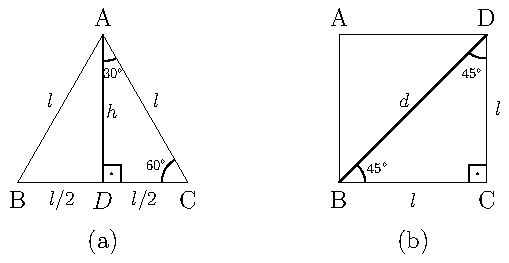
\includegraphics[scale=1.4]{Imagens/fig02.pdf}
        \caption{triângulo (a) e quadrado (b) utilizados para calcular o valor de seno, cosseno e tangente dos ângulos de 30°, 45° e 60° (ângulos notáveis).}
        \label{fig:02}
    \end{figure}

É possível calcular o seno de $30 \degree$ utilizando a fórmula do seno apresentada na equação \ref{eq:01}:
\[
\sen 30 \degree = \dfrac{\frac{l}{2}}{l} = \dfrac{l}{2} \cdot \dfrac{1}{l} = \dfrac{1}{2}
\]

Antes de calcular o cosseno e a tangente de $30 \degree$, é necessário  calcular a altura $h$ do $\Delta ABC$. Para isso, usa-se o teorema de Pitágoras:
\[
l^2 = h^2 + \left(\dfrac{l}{2}\right)^2 \Rightarrow l^2 = h^2 + \dfrac{l^2}{4} \Rightarrow h^2 = \dfrac{3l^2}{4} \Rightarrow h = \dfrac{l\sqrt{3}}{2}.
\]

Em seguida, é possível calcular o cosseno e a tangente de $30 \degree$ através das equações \ref{eq:02} e \ref{eq:03}, respectivamente:

\[
\cos 30 \degree = \dfrac{h}{l} = \dfrac{\dfrac{l\sqrt{3}}{3}}{l} =  \dfrac{l\sqrt{3}}{2} \cdot \dfrac{1}{l} = \dfrac{\sqrt{3}}{2} \; \text{e} \; \tg 30 \degree = \dfrac{\dfrac{l}{2}}{h} =  \dfrac{\dfrac{l}{2}}{\dfrac{l\sqrt{3}}{2}} = \dfrac{l}{2} \cdot \dfrac{2}{l\sqrt{3}} = \dfrac{1}{\sqrt{3}} = \dfrac{\sqrt{3}}{3}
\]

Procedimento análogo pode ser realizado para calcular os valores de seno, cosseno e tangente de $45 \degree$, considerando o quadrado ABCD, e $60 \degree$, considerando o triângulo ABC. A Tabela \ref{tab:01} apresenta os valores de seno, cosseno e tangente dos ângulos notáveis.

%%%%%%%%%%%% TABELA ÂNGULOS NOTÁVEIS %%%%%%%%%%%%
\begin{center}
 %{\fontfamily{helvet}\selectfont Valores de seno, cosseno e tangente de ângulos notáveis.}
 \end{center}
 \vspace{-0.2cm}
\begin{table}[!h]
    \centering     
    \caption{Valores de seno, cosseno e tangente de ângulos notáveis.}
    \begin{tabular}{p{0.12\textwidth}p{0.12\textwidth}p{0.12\textwidth}p{0.12\textwidth}}
\hline
 \begin{center}
     $\alpha$
 \end{center} 
 & 
 \begin{center}
     $\sen \alpha$ 
 \end{center}
 & 
 \begin{center}
     $\cos \alpha$ 
 \end{center}
 & 
 \begin{center}
     $\tg \alpha$
 \end{center}
 \\[-0.4cm]
\hline
 \begin{center}
     $30 \degree$ 
 \end{center}
 & 
 \begin{center}
     $\df{1}{2}$ 
 \end{center}
 & 
 \begin{center}
     $\df{\sqrt{3}}{2}$ 
 \end{center}
 & 
 \begin{center}
     $\df{\sqrt{3}}{3}$
 \end{center}\\[0.35cm]
 \begin{center}
     $45 \degree$ 
 \end{center}
 & 
 \begin{center}
     $\df{\sqrt{2}}{2}$ 
 \end{center}
 & 
 \begin{center}
     $\df{\sqrt{2}}{2}$ 
 \end{center}
 & 
 \begin{center}
     $1$ 
 \end{center}\\[0.35cm]
 \begin{center}
     $60 \degree$
 \end{center} 
 & \begin{center}
     $\df{\sqrt{3}}{2}$
 \end{center} 
 & 
 \begin{center}
     $\df{1}{2}$ 
 \end{center}
 & 
 \begin{center}
     $\sqrt{3}$
 \end{center}\\%[0.15cm]
\hline
\end{tabular}
\label{tab:01}
\end{table}

\subsection{Lei dos senos e lei dos cossenos}

 A lei dos senos e a lei dos cossenos são resultados importantes da trigonometria para estabelecer relações que auxiliam no cálculo dos ângulos e dos lados de triângulos quaisquer (triângulos retângulos, acutângulos e obtusângulos).

\noindent
 \textbf{Lei dos senos:} Em qualquer triângulo ABC (triângulo retângulo ou não), as medidas dos lados são proporcionais aos senos dos ângulos opostos, ou seja,
 $$\df{a}{\sen \hat{A}} = \df{b}{\sen \hat{B}} = \df{c}{\sen \hat{C}}$$

\noindent
\textbf{Exercício Resolvido}

Em um triângulo isósceles, tem-se a base medindo 9 cm e o ângulo oposto a base medindo $120 \degree$. Calcule a medida dos lados congruentes do triângulo.\\

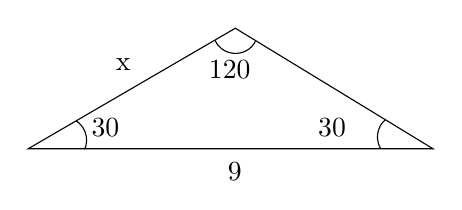
\begin{tikzpicture}[x=0.75pt,y=0.75pt,yscale=-0.65,xscale=0.65]

\draw   (343.49,20.56) -- (490,109.88) -- (190,109.88) -- cycle ;
%Shape: Arc [id:dp8670513073235429] 
\draw  [draw opacity=0] (358.59,29.81) .. controls (355.84,36.02) and (349.03,39.99) .. (341.63,39.1) .. controls (335.6,38.38) and (330.72,34.63) .. (328.46,29.66) -- (343.49,23.56) -- cycle ; \draw   (358.59,29.81) .. controls (355.84,36.02) and (349.03,39.99) .. (341.63,39.1) .. controls (335.6,38.38) and (330.72,34.63) .. (328.46,29.66) ;  
%Shape: Arc [id:dp6736551053433504] 
\draw  [draw opacity=0] (451.18,109.7) .. controls (449.44,106.76) and (448.58,103.21) .. (448.94,99.48) .. controls (449.4,94.83) and (451.66,90.82) .. (454.92,88.14) -- (464.52,101) -- cycle ; \draw   (451.18,109.7) .. controls (449.44,106.76) and (448.58,103.21) .. (448.94,99.48) .. controls (449.4,94.83) and (451.66,90.82) .. (454.92,88.14) ;  
%Shape: Arc [id:dp020705992733369705] 
\draw  [draw opacity=0] (225.63,89.28) .. controls (228.49,91.15) and (230.83,93.95) .. (232.16,97.45) .. controls (233.81,101.82) and (233.56,106.42) .. (231.83,110.27) -- (217.52,103) -- cycle ; \draw   (225.63,89.28) .. controls (228.49,91.15) and (230.83,93.95) .. (232.16,97.45) .. controls (233.81,101.82) and (233.56,106.42) .. (231.83,110.27) ;  

% Text Node
\draw (235,86) node [anchor=north west][inner sep=0.75pt]   [align=left] {$30 \degree$};
% Text Node
\draw (403,86) node [anchor=north west][inner sep=0.75pt]   [align=left] {$30 \degree$};
% Text Node
\draw (322,43) node [anchor=north west][inner sep=0.75pt]   [align=left] {$120  \degree$};
% Text Node
\draw (253,41) node [anchor=north west][inner sep=0.75pt]   [align=left] {x};
% Text Node
\draw (336,118) node [anchor=north west][inner sep=0.75pt]   [align=left] {9};
\end{tikzpicture}
\hfill
\begin{minipage}{8.2cm}
\vspace{-1.5cm}

\noindent
Pela lei dos senos, temo:\\
\[
\frac{9}{\sen 120 \degree}=\frac{x}{\sen 30 \degree}=\frac{x}{\frac{\sqrt{3}}{2}}=\frac{x}{\frac{1}{2}}\Rightarrow x=3 \sqrt{3} \text{cm}
\]
\end{minipage}

\noindent
\textbf{Lei dos cossenos:} Em qualquer triângulo ABC (triângulo retângulo ou não), o quadrado da medida de um lado é igual à soma dos quadrados das medidas dos outros lados menos duas vezes o produto das medidas desses lados pelo cosseno do ângulo que eles formam, ou seja,

$$a^2 = b^2 + c^2 -2bc\cdot\cos\hat{A}$$
$$b^2 = a^2 + c^2 -2ac\cdot\cos\hat{B}$$
$$c^2 = a^2 + b^2 -2ab\cdot\cos\hat{C}$$

\noindent
\textbf{Exercício resolvido} \\
\begin{minipage}{0.5\textwidth}
    Determine a medida de a no triângulo ilustrado na figura a seguir.
\end{minipage}
\vspace{1cm}
\begin{minipage}{0.5\textwidth}
\vspace{1cm}
\centering
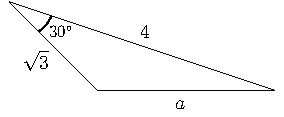
\includegraphics[width=0.8\textwidth]{Imagens/fig04.pdf}
\end{minipage}
Resolução:
\[
a^2=b^2+c^2-2 \cdot b \cdot c \cdot \cos \hat{A} = 4^2+(\sqrt{3})^2-2 \cdot 4 \cdot \sqrt{3} \cdot \cos 30 \degree = 16 + 3 -8 \sqrt{3} \cdot \dfrac{\sqrt{3}}{2}=7
\]
\[
\Rightarrow a=\sqrt{7}
\]

\subsection{Arcos e ângulos}

Algumas definições para o estudo de trigonometria na circunferência são fornecidas a seguir.\\
\begin{center}
\begin{minipage}{6cm}
        \centering
            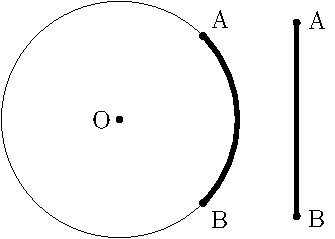
\includegraphics[width=1.2\textwidth]{Imagens/fig05.pdf}
            \captionof{figure}{O arco $\wideparen{AB}$ e comprimento desse arco dado pela medida algébrica do segmento $\overline{AB}$.}
            \label{fig:fig05}
\end{minipage}
\end{center}

\noindent
\textbf{Arco geométrico:} é uma das partes da circunferência delimitada por dois pontos, incluindo-os.

\noindent
\textbf{Comprimento de um arco:} é o comprimento do segmento de reta que se obtém ao “desentortar” (ou retificar) o arco. Conhecendo o raio da circunferência e a medida em graus do arco, o comprimento do arco pode ser calculado através de uma regra de três simples:\\

\begin{center}
\begin{tabular}{rcl}
Graus    &        & Comprimento do arco   \\
$360$    & ------ & $2 \pi r$      \\
$\alpha$ & ------ & $x$        \\
\end{tabular}
\end{center}

Nesse caso, o comprimento $x$ é expresso na mesma unidade do raio da circunferência. Em uma circunferência de raio $r=1$, a regra de três acima é simplificada da seguinte forma:

\begin{center}
\begin{tabular}{rcl}
Graus    &        & Comprimento do arco   \\
$180$    & ------ & $\pi$      \\
$\alpha$ & ------ & $x$        \\
\end{tabular}
\end{center}

\noindent
\textbf{Medida em radianos:} Observe na Figura \ref{fig:fig06} que os arcos $\wideparen{AB}$, $\wideparen{CD}$ e $\wideparen{EF}$ têm a mesma medida em graus, porém têm comprimentos diferentes. Utilizando a regra de três acima, tem-se que:

\begin{minipage}{5cm}
    \[
    x_1=\dfrac{\pi r_1}{6} \;\;\; x_2=\dfrac{\pi r_2}{6} \;\;\; x_3=\dfrac{\pi r_3}{6}
    \]
\end{minipage}
\hfill
\begin{minipage}{8cm}
        \centering
            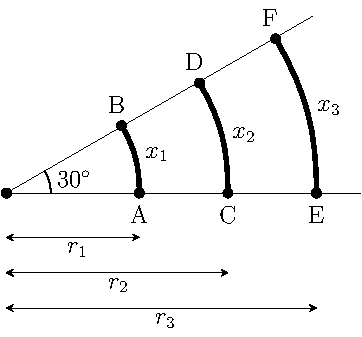
\includegraphics[width=0.8\textwidth]{Imagens/fig06.pdf}
            \captionof{figure}{Arco com raios diferentes.}
            \label{fig:fig06}
\end{minipage}

\vspace{1cm}
Note que $\dfrac{x_1}{r_1}=\dfrac{x_2}{r_2}=\dfrac{x_3}{r_3}=\dfrac{\pi}{6}$. A razão entre o comprimento do arco e o raio, que nesse exemplo é $\dfrac{\pi}{6}$, é a \textbf{medida em radianos} do arco (e também do ângulo central).

\subsection{Circunferência trigonométrica}
Passa-se a utilizar a circunferência unitária (ou circunferência trigonométrica), uma circunferência com raio igual a 1 unidade de comprimento associada a um sistema de coordenadas cartesianas ortogonais rOs, conforme a Figura \ref{fig:fig07e08} (a). Os pontos A,B,C e D, intersecções da circunferência trigonométrica com os eixos coordenados, dividem a circunferência em quatro partes congruentes denominadas \textbf{quadrantes}.

\begin{minipage}{13.5cm}
     \centering
\begin{minipage}{6cm}
     \centering
            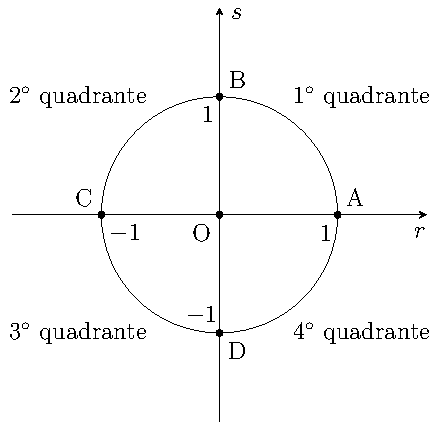
\includegraphics[width=\textwidth]{Imagens/fig07.pdf}
\end{minipage}
\hfill
\begin{minipage}{6cm}
        \centering
            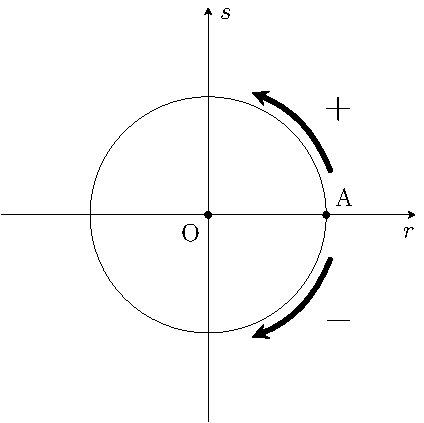
\includegraphics[width=\textwidth]{Imagens/fig08.pdf}
\end{minipage}
\captionof{figure}{Circunferência trigonométrica e seus quadrantes (a); sentidos da circunferência trigonométrica (b).}
\label{fig:fig07e08}
\end{minipage}


Podemos associar a cada número real $x$ um ponto da circunferência trigonométrica. Ao número $x=0$, associamos o ponto A. Se $x \neq 0$, associamos a $x$ o ponto final $P$ do seguinte percurso de comprimento igual a $|x|$ realizado sobre a circunferência partindo de $A$, de acordo com a Figura \ref{fig:fig07e08} (b):

\begin{itemize}
    \item 	Se $x>0$, percorremos a circunferência trigonométrica no sentido anti-horário;
    \item 	Se $x<0$, percorremos a circunferência trigonométrica no sentido horário.
\end{itemize}

O ponto $P$ associado à $x$ é denominado \textbf{imagem de $x$} na circunferência trigonométrica e o arco $\wideparen{AP}$ tem $x$ rad.

\noindent
\textbf{Exercício Resolvido:} Marcar na circunferência trigonométrica a imagem do número $x$ em cada caso:

\begin{tasks}(4)
    \task $x=\dfrac{\pi}{2}$
    \task $x=1$
    \task $x=-1$
    \task $x=-\dfrac{2 \pi}{3}$
\end{tasks}
\noindent
Resolução:\\
\begin{minipage}{\textwidth}
     \centering
\begin{minipage}{0.24\textwidth}
     \centering
            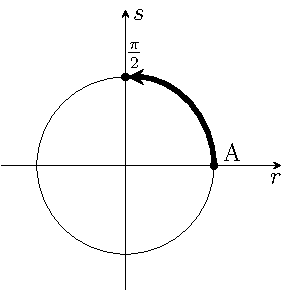
\includegraphics[width=\textwidth]{Imagens/fig09.pdf}
\end{minipage}
\begin{minipage}{0.24\textwidth}
        \centering
            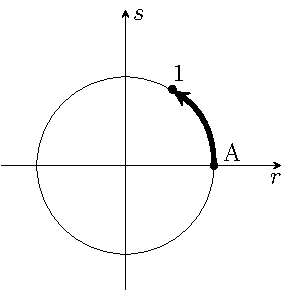
\includegraphics[width=\textwidth]{Imagens/fig10.pdf}
\end{minipage}
\begin{minipage}{0.24\textwidth}
     \centering
            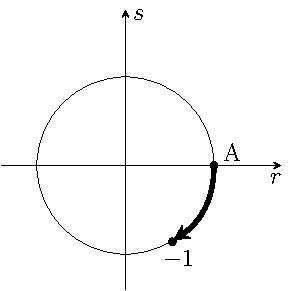
\includegraphics[width=\textwidth]{Imagens/fig11.pdf}
\end{minipage}
\begin{minipage}{0.24\textwidth}
        \centering
            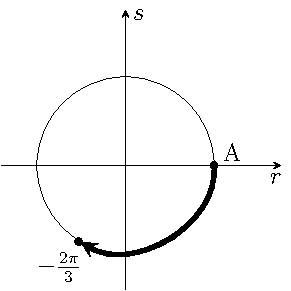
\includegraphics[width=\textwidth]{Imagens/fig12.pdf}
\end{minipage}
\end{minipage}

Se o ponto da circunferência, final do arco iniciado em (1,0), é o mesmo para dois arcos diferentes, então chamamos estes arcos de \textbf{arcos côngruos} (ou congruentes). Observe que todos os arcos côngruos diferem si de um múltiplo de $2\pi$ rad (ou $360\degree$), que é o comprimento de cada volta. Dessa forma, os arcos ($x+k \cdot 2\pi$) rad (ou $\alpha+k \cdot 360\degree$), para $k \in \mathbb{Z}$, são côngruos.\\

\noindent
\textbf{Exercício Resolvido:} Dentre os arcos abaixo, identifique os côngruos:

\begin{tasks}(2)
    \task $30 \degree \;\; \text{e} \;\; 330 \degree$
    \task $\dfrac{\pi}{3} \text{rad} \;\; \text{e} \;\; \dfrac{31 \pi}{3} \text{rad}  $
\end{tasks}
\noindent
Resolução:\\
 
\begin{tasks}
    \task 	Encontrar $k \in \mathbb{Z}$, tal que $30 + k \cdot 360 \degree = 330 \degree \Rightarrow k = \dfrac{5}{6} \not \in Z \Rightarrow 30 \degree$ e $330 \degree$ não são côngruos.
    \task 	Encontrar $k \in \mathbb{Z}$, tal que $\dfrac{\pi}{3} + 2k \pi = \dfrac{31 \pi}{3} \Rightarrow k = 5 \in Z \Rightarrow \dfrac{\pi}{3} \text{rad e }\dfrac{31 \pi}{3} \text{rad}$ são côngruos.
\end{tasks}

\subsection{Seno e cosseno na circunferência trigonométrica}

Dado  $x \in \mathbb{R}$ com imagem de $x$ na circunferência trigonométrica sendo um ponto com coordenadas $(a,b)$, definimos:

\begin{tcolorbox}[colback=white,colframe=minha_cor,coltitle=black,title=Definição: Seno e cosseno] 
\[
\cos x = a \text{  e  } \sen x = b
\]
\end{tcolorbox}

Dessa forma, passa-se a chamar o eixo das abscissas de \textbf{eixo dos cossenos} e o eixo das ordenadas de \textbf{eixo dos senos}, conforme a Figura \ref{fig:fig13}.
\begin{center}
    \begin{minipage}{7cm}
        \centering
            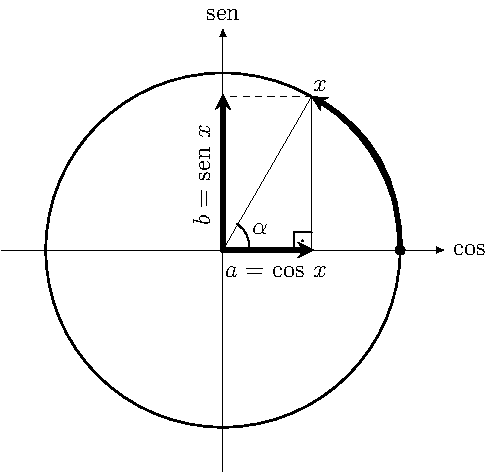
\includegraphics[width=1.2\textwidth]{Imagens/fig13.pdf}
            \captionof{figure}{Circunferência trigonométrica e sua relação com seno e cosseno de um número real $x$.}
            \label{fig:fig13}
    \end{minipage}
\end{center}

Nota-se que as definições de seno e cosseno de um ângulo agudo em um triângulo retângulo são coerentes com as definições na circunferência trigonométrica:
\[
\sen \alpha = \dfrac{\text{medida do cateto oposto}}{\text{medida da hipotenusa}} = \dfrac{b}{1} = b = \sen x
\]
\[
\cos \beta = \dfrac{\text{medida do cateto adjacente}}{\text{medida da hipotenusa}} = \dfrac{a}{1} = a = \cos x
\]

Os valores de seno e cosseno das medidas de arcos dadas em graus são iguais aos valores de seno e cosseno dos números reais que se obtêm transformando essas medidas em radianos.

Além disso, utilizando propriedades de simetria em relação aos eixos coordenados, obtém-se os arcos e seus correspondentes valores de seno e cosseno, conforme a circunferência trigonométrica apresentada na Figura \ref{fig:fig05_circtrigcompl}.

\begin{figure}[h]
        \centering
        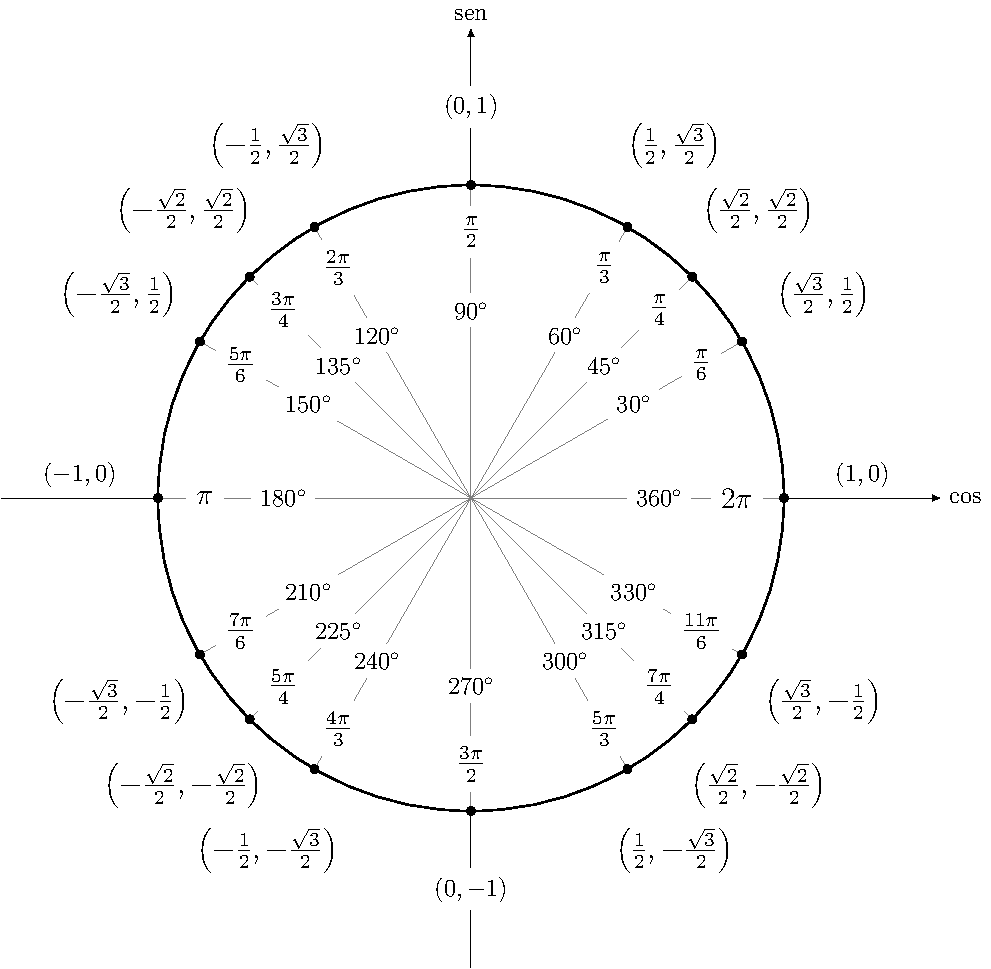
\includegraphics[width=\textwidth]{Imagens/fig05_circtrigcompl.pdf}
        \caption{Circunferência trigonométrica com os principais arcos (em graus e em radianos) e seus correspondentes valores de seno e cosseno apresentados em pares de coordenadas.}
        \label{fig:fig05_circtrigcompl}
 \end{figure}

Nota-se que dois arcos côngruos possuem senos iguais e cossenos iguais. Em outras palavras, para todo $x \in \mathbb{R}$ e para todo $k \in \mathbb{Z}$, temos:
\[
\sen (x + 2 k \pi) = \sen x
\]
\[
\cos (x + 2 k \pi) = \cos x
\]

\noindent
\textbf{Exercício resolvido} 

Calcule o valor da expressão
\[
\dfrac{\cos \dfrac{7 \pi}{6}-\sen \dfrac{\pi}{3}}{\sen \left(-\dfrac{\pi}{4}\right) + \cos \dfrac{19 \pi}{3}}
\]

\noindent
Resolução:
\[
\dfrac{\cos \dfrac{7 \pi}{6}-\sen \dfrac{\pi}{3}}{\sen \left(-\dfrac{\pi}{4}\right) + \cos \dfrac{19 \pi}{3}} = \dfrac{- \dfrac{\sqrt{3}}{2} - \dfrac{\sqrt{3}}{2}}{- \dfrac{\sqrt{2}}{2} + \dfrac{1}{2}} = \dfrac{- 2 \sqrt{3}}{1 - \sqrt{2}} = \dfrac{ 2 \sqrt{3}}{\sqrt{2}-1} \cdot \dfrac{\sqrt{2}+1}{\sqrt{2}+1} = 2 \sqrt{6} + 2 \sqrt{3}
\]
\textbf{Tangente na circunferência trigonométrica}

Pelo ponto $A$, origem da circunferência trigonométrica, a reta $t$ paralela ao eixo dos senos é traçada e orientada no mesmo sentido dele. Dado um número real $x$ com imagem no ponto $P$ da circunferência trigonométrica, tal que a reta $\overleftrightarrow{OP}$ intercepta o eixo das tangentes no ponto $T$, define-se $\tg x$ a medida algébrica do segmento $\overline{AT}$, que será positiva quando $T$ estiver “acima” de $A$, e negativa quando $T$ estiver “abaixo” de $A$. Dessa forma, passa-se a chamar a reta $t$ de \textbf{eixo das tangentes}, conforme a Figura \ref{fig:fig14}.
\begin{center}
    \begin{minipage}{10cm}
        \centering
            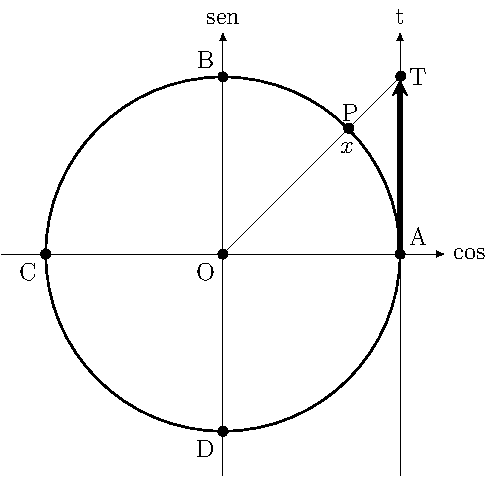
\includegraphics[width=0.7\textwidth]{Imagens/fig14.pdf}
            \captionof{figure}{Circunferência trigonométrica com o eixo das tangentes.}
            \label{fig:fig14}
    \end{minipage}
\end{center}

Observe que, quando $P=B$ ou $P=D$, a reta $\overleftrightarrow{OP}$ é paralela ao eixo das tangentes e, portanto, não existe o ponto $T$. Nesse caso, não existe $\tg x$. Então,
\[
x \neq \dfrac{(2 k + 1) \pi}{2}, \;\; k \in \mathbb{Z} \Longrightarrow  \exists \tg x 
\]
\section{Funções trigonométricas}	

A seguir, os conceitos visto até aqui serão formalizados sob o ponto de vista de funções matemáticas.

\subsection{Estudo da função seno}

Dado um número real $x$, associa-se a ele o valor do seno de um arco de $x$ radianos. Assim, define-se a função seno como a função real de variável real que associa a cada número real $x$ o valor real $\sen x$, ou seja,
\begin{center}
    \begin{tabular}{llll}
    $f:$ & $\mathbb{R}$ & $\rightarrow$ & $\mathbb{R}$\\
    & $x$ & $\mapsto$ & $f(x) = \sen x$\\
\end{tabular}    
\end{center}

A partir de valores de $x$ da primeira volta positiva na circunferência trigonométrica (esses valores foram apresentados anteriormente na Figura \ref{fig:fig05_circtrigcompl}), constrói-se o gráfico da função seno apresentado abaixo. %na Figura \ref{fig:fig16}.

%\begin{center}
%    \begin{minipage}{14cm}
%        \centering
%            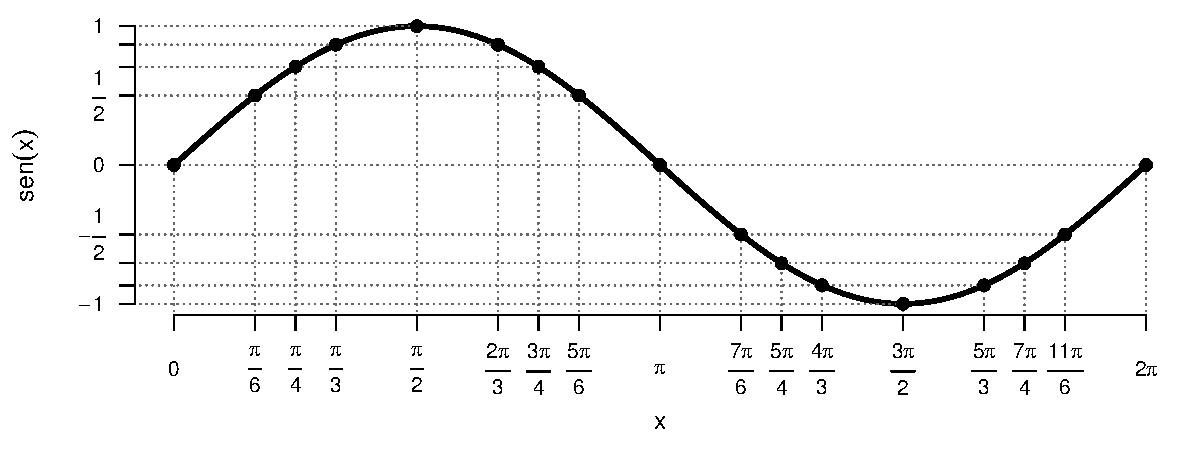
\includegraphics[width=\textwidth]{Imagens/fig16.pdf}
%            \captionof{figure}{Gráfico da função seno para $x \in [0,2 \pi]$.}
%            \label{fig:fig16}
%    \end{minipage}
%\end{center}


%%%%%%%%%%%%%%%%%%%%%%%%%%%%%%%%%%%%%%	
\begin{center}
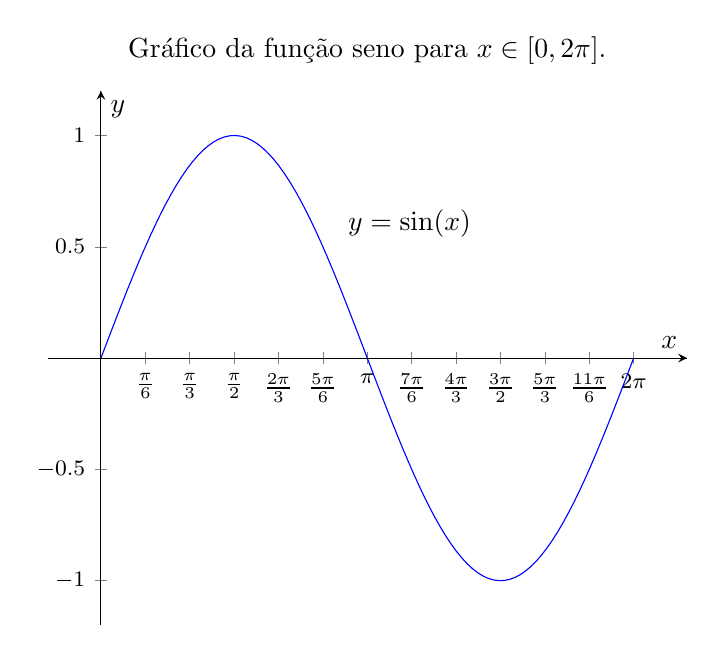
\begin{tikzpicture}
\begin{axis}[
width=0.8\textwidth,
xlabel=$x$,
ylabel=$y$,
title={Gráfico da função seno para $x \in [0,2 \pi]$.},
axis lines=middle,
xmin=0,
xmax=2*pi,
ymin=-1,
ymax=1,
xtick={0,pi/6,pi/3,pi/2,2*pi/3,5*pi/6,pi,7*pi/6,4*pi/3,3*pi/2,5*pi/3,11*pi/6,2*pi},
xticklabels={$0$,$\frac{\pi}{6}$,$\frac{\pi}{3}$,$\frac{\pi}{2}$,$\frac{2\pi}{3}$,$\frac{5\pi}{6}$,$\pi$,$\frac{7\pi}{6}$,$\frac{4\pi}{3}$,$\frac{3\pi}{2}$,$\frac{5\pi}{3}$,$\frac{11\pi}{6}$,$2\pi$},
ytick={-1,-0.5,0,0.5,1},
enlargelimits,
ticks=both,
tick label style={font=\footnotesize},
after end axis/.code={
\draw (axis cs:0,\pgfkeysvalueof{/pgfplots/ymin}) -- (axis cs:0,\pgfkeysvalueof{/pgfplots/ymax});
\draw (axis cs:\pgfkeysvalueof{/pgfplots/xmin},0) -- (axis cs:\pgfkeysvalueof{/pgfplots/xmax},0);
\node[black, above right] at (axis cs:2.8,0.5) {$y =\sin(x)$};
}
]
\addplot[domain=0:2*pi, blue, samples=100] {sin(deg(x))};
\end{axis}
\end{tikzpicture}
\end{center}


            



Nota-se que a função seno é definida no conjunto dos números reais. Assim, a curva pode ser estendida para valores de $x$ menores do que 0 e maiores do que $2 \pi$.

\textbf{Observações sobre a função seno:}
\begin{itemize}
    \item 	O domínio de $f(x)= \sen x$ é $D(f) = \mathbb{R}$, pois para qualquer valor real de $x$ existe um e, somente um, valor para $\sen x$.
    \item   O conjunto imagem de $f(x)= \sen x$ é o intervalo $[-1,1]$.
    \item   A função seno não é sobrejetiva, pois sua imagem não é igual ao contradomínio, isto é, $Im(f)=[-1,1] \neq \mathbb{R} = CD(f)$.
    \item   A função seno não é injetiva, pois, para valores diferentes de $x$, temos o mesmo $f(x)$.
    \item   A função seno é uma função ímpar, isto é, qualquer que seja $x \in D(f) = \mathbb{R} $, tem-se que $\sen x = - \sen (-x)$.
    \item   A função seno é periódica com período igual à $ 2 \pi$, isto é, $\sen x = \sen (x+2k \pi)$, com $k \in \mathbb{R} e x \in \mathbb{R}$.
\end{itemize}
\subsection{Estudo da função cosseno}

Dado um número real $x$, associa-se a ele o valor do cosseno de um arco de $x$ radianos. Assim, a função cosseno é definida como a função real de variável real que associa a cada número real $x$ o valor real $\cos x$, ou seja,
\begin{center}
\begin{tabular}{llll}
$f:$ & $\mathbb{R}$ & $\rightarrow$ & $\mathbb{R}$\\
   & $x$ & $\mapsto$ & $f(x) = \cos x$\\
\end{tabular}
\end{center}

A partir de valores de $x$ da primeira volta positiva na circunferência trigonométrica (esses valores foram apresentados anteriormente na Figura \ref{fig:fig05_circtrigcompl}), constrói-se o gráfico da função cosseno apresentado abaixo. %na Figura \ref{fig:fig17}.
%\begin{center}
%    \begin{minipage}{14cm}
%        \centering
%            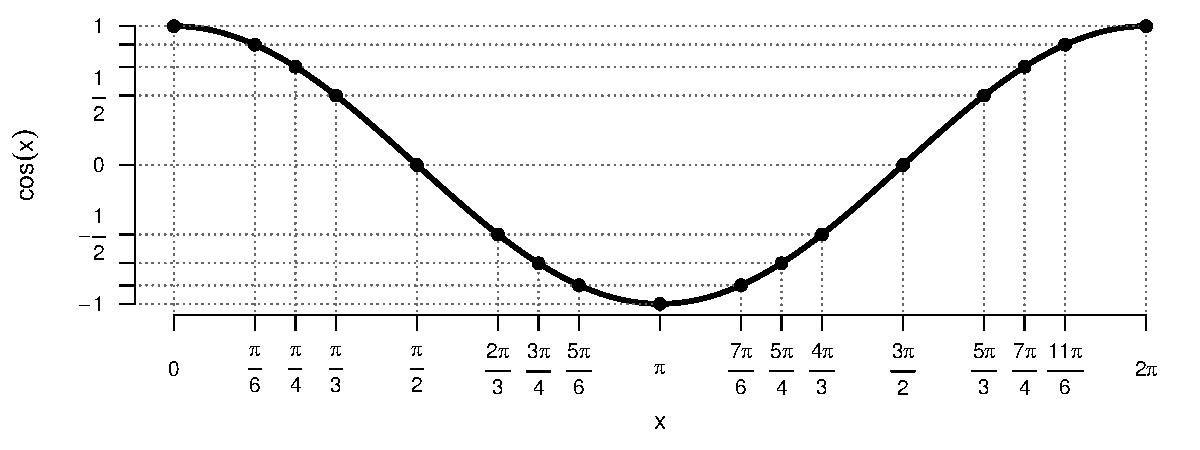
\includegraphics[width=\textwidth]{Imagens/fig17.pdf}
%            \captionof{figure}{Gráfico da função cosseno para $x %\in [0,2 \pi]$.}
%            \label{fig:fig17}
%    \end{minipage}
%\end{center}

%%%%%%%%%%%%%%%%%%%%%%%%%%%%%%%%%%%%%%	
\begin{center}
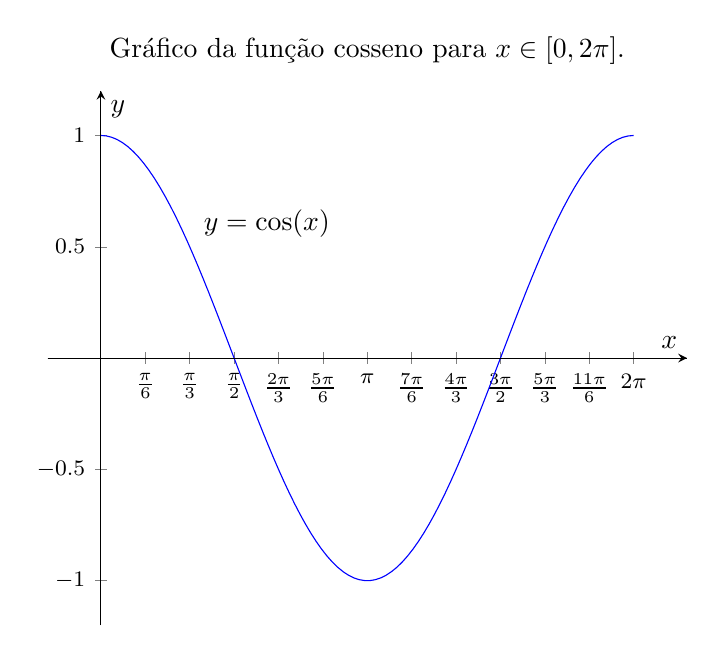
\begin{tikzpicture}
\begin{axis}[
width=0.8\textwidth,
xlabel=$x$,
ylabel=$y$,
title={Gráfico da função cosseno para $x \in [0,2 \pi]$.},
axis lines=middle,
xmin=0,
xmax=2*pi,
ymin=-1,
ymax=1,
xtick={0,pi/6,pi/3,pi/2,2*pi/3,5*pi/6,pi,7*pi/6,4*pi/3,3*pi/2,5*pi/3,11*pi/6,2*pi},
xticklabels={$0$,$\frac{\pi}{6}$,$\frac{\pi}{3}$,$\frac{\pi}{2}$,$\frac{2\pi}{3}$,$\frac{5\pi}{6}$,$\pi$,$\frac{7\pi}{6}$,$\frac{4\pi}{3}$,$\frac{3\pi}{2}$,$\frac{5\pi}{3}$,$\frac{11\pi}{6}$,$2\pi$},
ytick={-1,-0.5,0,0.5,1},
enlargelimits,
ticks=both,
tick label style={font=\footnotesize},
after end axis/.code={
\draw (axis cs:0,\pgfkeysvalueof{/pgfplots/ymin}) -- (axis cs:0,\pgfkeysvalueof{/pgfplots/ymax});
\draw (axis cs:\pgfkeysvalueof{/pgfplots/xmin},0) -- (axis cs:\pgfkeysvalueof{/pgfplots/xmax},0);
\node[black, above right] at (axis cs:1.1,0.5) {$y =\cos(x)$};
}
]
\addplot[domain=0:2*pi, blue, samples=100] {cos(deg(x))};
\end{axis}
\end{tikzpicture}
\end{center}


Similarmente à função seno, a curva da função cosseno pode ser estendida para valores de $x$ menores do que 0 e maiores do que $2 \pi$.

\textbf{Observações sobre a função cosseno:}
\begin{itemize}
   \item O domínio e a imagem da função cosseno são os mesmos da função seno.
    \item Assim como a função seno, a função cosseno não é nem sobrejetiva nem injetiva.
    \item A função cosseno é uma função par, isto é, qualquer que seja $x\in \text{D}(f)$, temos que $\cos x= \cos (-x)$.
    \item A função cosseno é periódica com período igual à $2\pi$.
\end{itemize}

\subsection{Estudo da função tangente}

Define-se função tangente como a função real de variável real que associa a cada número $x$ o valor $\tg x$, desde que $x$ não seja $\frac{\pi}{2}$ nem $\frac{3\pi}{2}$ e nenhum de seus respectivos arcos côngruos, isto é,

\begin{center}
\begin{tabular}{llll}
$f:$ & $\mathbb{D}$ & $\rightarrow$ & $\mathbb{R}$\\
   & $x$ & $\mapsto$ & $f(x) = \tg x$\\
\end{tabular}
\end{center}
em que $\mathbb{D} = \left\{x \in \mathbb{R} \ | \ x \neq \df{(2k+1)\pi}{2}, \text{com} \ k \in \mathbb{Z}\right\}$

A partir de valores de $x$ da primeira volta positiva na circunferência trigonométrica (esses valores foram apresentados anteriormente na Figura \ref{fig:fig05_circtrigcompl}), constrói-se o gráfico da função tangente apresentado abaixo. % na Figura \ref{fig:fig18}.
%\begin{center}
%    \begin{minipage}{14cm}
%        \centering
%            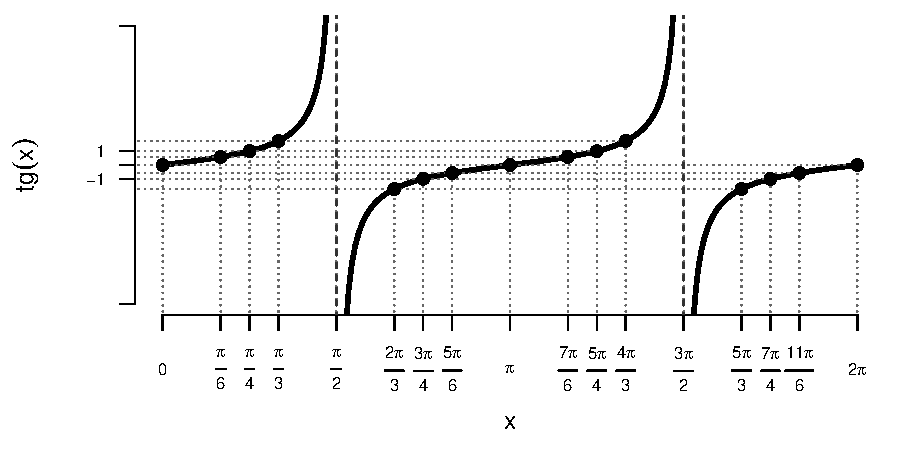
\includegraphics[width=\textwidth]{Imagens/fig18.pdf}
%            \captionof{figure}{Gráfico da função tangente para $x \in [0,2 \pi]$.}
%            \label{fig:fig18}
%    \end{minipage}
%\end{center}

%%%%%%%%%%%%%%%%%%%%%%%%%%%%%%%%%%%%%%%%%%%%%%%%
\begin{center}
\begin{tikzpicture}
\begin{axis}[
restrict y to domain=-10:10,
samples=1000,
% some fine-tuning for the display:
width=17cm, height=220pt,
xlabel=$x$,
ylabel=$\tg(x)$,
title={Gráfico da função tangente para $x \in [-2 \pi,2 \pi]$.},
xmin=-2.2*pi, xmax=2.2*pi,
xtick={-2*pi,-3*pi/2,...,2*pi},
xticklabels={$-2\pi$,$-\frac{11\pi}{6}$,$-\frac{5\pi}{3}$,$-\frac{3\pi}{2}$,$-\frac{4\pi}{3}$,$-\pi$,$\frac{7\pi}{6}$,$-\frac{5\pi}{6}$,$-\frac{2\pi}{3}$,$-\frac{\pi}{2}$,$-\frac{\pi}{3}$,$-\frac{\pi}{6}$,$0$,$\frac{\pi}{6}$,$\frac{\pi}{3}$,$\frac{\pi}{2}$,$\frac{2\pi}{3}$,$\frac{5\pi}{6}$,$\pi$,$\frac{7\pi}{6}$,$\frac{4\pi}{3}$,$\frac{3\pi}{2}$,$\frac{5\pi}{3}$,$\frac{11\pi}{6}$,$2\pi$},
axis x line=center,
axis y line=center,
]
\addplot [blue] gnuplot [id=tangens,domain=-2*pi:2*pi] {tan(x)};
\draw[dashed] (-3*pi/2,-10) -- (-3*pi/2,10);
\draw[dashed] (-pi/2,-10) -- (-pi/2,10);
\draw[dashed] (pi/2,-10) -- (pi/2,10);
\draw[dashed] (3*pi/2,-10) -- (3*pi/2,10);
%\legend{$\tan(x)$}
\end{axis}
\end{tikzpicture}
\end{center}
%%%%%%%%%%%%%%%%%%%%%%%%%%%%%%%%%%%%%%%%%%%

Nota-se que à medida que $x$ tende aos valores $\frac{\pi}{2}, \frac{3\pi}{2}$ e seus respectivos arcos côngruos, o gráfico da tangente tende ao infinito (positivo ou negativo). A curva da função tangente pode ser estendida para valores de $x$ menores do que $0$ e maiores do que $2\pi$.

\textbf{Observações sobre a função tangente:}
\begin{itemize}
   \item A função tangente tem $\text{D}(f)=\left\{x \in \mathbb{R} \ | \ x \neq \frac{(2k+1)\pi}{2}, \text{com} \ k \in \mathbb{Z}\right\}$ e $\text{Im}(f)=\mathbb{R}$.
    \item A função tangente não é injetiva, mas é sobrejetiva.
    \item A função tangente é função ímpar, isto é, $\tg x= -\tg (-x),\forall x\in \text{D}(f)$.
    \item A função tangente é periódica com período igual à $\pi$, isto é, $\tg x=\tg (x+k\pi), \text{com} \ k\in \mathbb{Z}$ e $x\in \text{D}(f)$.
\end{itemize}

\section{Relações e transformações trigonométricas}

As relações e transformações trigonométricas são apresentadas a seguir.

\begin{tcolorbox}[colback=white,colframe=minha_cor,coltitle=black,title=Relações trigonométricas] 
    \begin{minipage}{6.5cm}
    \textbf{Relações principais:} \\[0.25cm]
    $\sen^2 x + \cos^2 x = 1$ \\[0.25cm]
    $\tg x = \df{\sen x}{\cos x}, \forall x \neq \df{(2k+1)\pi}{2}$ \\[0.25cm]
    $\cotg x = \df{\cos x}{\sen x}, \forall x \neq k\pi$ \\[0.25cm]
    $\sec x = \df{1}{\cos x}, \forall x \neq \df{(2k+1)\pi}{2}$ \\[0.25cm]
    $\cossec x = \df{1}{\sen x}, \forall x \neq k\pi$
\end{minipage}
\hfill
\begin{minipage}{6.5cm}
    \textbf{Relações decorrentes:} \\[0.25cm]
    $\cotg x = \df{1}{\tg x}, \forall x \neq \df{k\pi}{2}$ \\[0.25cm]
    $\sec^2x = 1 + \tg^2x, \forall x \neq \df{(2k+1)\pi}{2}$ \\[0.25cm]
    $\cossec^2x = 1 + \cotg^2x, \forall x \neq k\pi$\\[1.50cm]
\end{minipage}
\end{tcolorbox}

\begin{tcolorbox}[colback=white,colframe=minha_cor,coltitle=black,title=Soma de diferença de arcos] 
\begin{center}
    \begin{minipage}{6.5cm}
    $\sen (a \pm b) = \sen a \cdot \cos b \pm \sen b \cdot \cos a$ \\[0.25cm]
    $\cos (a \pm b) = \cos a \cdot \cos b \mp \sen a \cdot \cos b$ \\[0.25cm]
    $\tg (a \pm b) = \dfrac{\tg a \pm \tg b}{1 + tg a \cdot \tg b}$ \\
    \end{minipage}
\end{center}
\end{tcolorbox}

\begin{tcolorbox}[colback=white,colframe=minha_cor,coltitle=black,title=Divisão de arcos] 
\begin{center}
    \begin{minipage}{6.5cm}
    $\sen^2 \dfrac{x}{2} = \dfrac{1- \cos x}{2}$ \\[0.25cm]
    $\cos^2 \dfrac{x}{2} = \dfrac{1+ \cos x}{2}$ \\[0.25cm]
    $\tg^2 \dfrac{x}{2} = \dfrac{1- \cos x}{1+ \cos x}$ \\
    \end{minipage}
\end{center}
\end{tcolorbox}

\begin{tcolorbox}[colback=white,colframe=minha_cor,coltitle=black,title=Multiplicação de arcos] 
\begin{center}
    \begin{minipage}{6.5cm}
    $\sen 2a = 2 \cdot \sen a \cdot \cos a$ \\[0.25cm]
    $\cos 2a = \cos^2 a - \sen^2 a$ \\[0.25cm]
    $\tg 2a = \dfrac{2 \cdot \tg a}{1- \tg^2 a}$ \\
    \end{minipage}
\end{center}
\end{tcolorbox}

\begin{tcolorbox}[colback=white,colframe=minha_cor,coltitle=black,title=Transformação em produtos] 
\begin{center}
    \begin{minipage}{7cm}
    $\sen p + \sen q = 2 \cdot \sen \dfrac{p + q}{2} \cdot \cos \dfrac{p - q}{2}$ \\[0.25cm]
    $\sen p - \sen q = 2 \cdot \sen \dfrac{p - q}{2} \cdot \cos \dfrac{p + q}{2}$ \\[0.25cm]
    $\cos p + \cos q = 2 \cdot \cos \dfrac{p + q}{2} \cdot \cos \dfrac{p - q}{2}$ \\[0.25cm]
     $\cos p - \sen q = -2 \cdot \sen \dfrac{p + q}{2} \cdot \sen \dfrac{p - q}{2}$ \\
    \end{minipage}
\end{center}
\end{tcolorbox}

\begin{texample}
        \centering
        \tcbhighmath{\text{Seja } \sen x = \dfrac{2}{5} \text{  e  }  0 < x < \dfrac{\pi}{2}. \text{ Calcule } \cos x \text{  e  } \tg x.}
\end{texample}
Resolução:
\[\sen^2 x + \cos^2 x = 1 \Rightarrow \left(\dfrac{2}{5}\right)^2 + \cos^2 x = 1 \Rightarrow \cos^2 x  = \dfrac{21}{25}\Rightarrow \cos x =  
    \left\{  
         \begin{array}{c}
            \dfrac{-\sqrt{21}}{5} \\[0.3cm]
		  \dfrac{+\sqrt{21}}{5} \\
	\end{array} 
    \right. 
\]
\[
\Rightarrow \cos x = \dfrac{\sqrt{21}}{5} \text{ e } \tg x = \dfrac{\sen x}{\cos x} = \dfrac{\frac{2}{5}}{\frac{\sqrt{21}}{5}} = \dfrac{2 \sqrt{21}}{21}
\]

\begin{texample}
        \centering
        \tcbhighmath{\text{Calcule  valor da expressão } \sen 105 \degree - \cos 75 \degree}
\end{texample}
Resolução:
\[
\Rightarrow 105 \degree = 60 \degree + 45 \degree \text{ e } 75 \degree = 30 \degree + 45 \degree
\]
\[
\sen 105 \degree - \cos 75 \degree = \sen(60 \degree + 45 \degree) - \cos(30 \degree + 45 \degree) =
\]
\[
\dfrac{\sqrt{3}}{2} \cdot \dfrac{\sqrt{2}}{2} + \dfrac{\sqrt{2}}{2} \cdot \dfrac{1}{2} - \left[ \dfrac{\sqrt{3}}{2} \cdot \dfrac{\sqrt{2}}{2} - \dfrac{1}{2} \cdot  \dfrac{\sqrt{2}}{2}  \right] = \dfrac{\sqrt{6}}{4} + \dfrac{\sqrt{2}}{4} - \left[ \dfrac{\sqrt{6}}{4} - \dfrac{\sqrt{2}}{4} \right] =
\]
\[
\dfrac{\sqrt{6}}{4} + \dfrac{\sqrt{2}}{4} -  \dfrac{\sqrt{6}}{4} + \dfrac{\sqrt{2}}{4} =
\dfrac{2 \sqrt{2}}{4} = \dfrac{\sqrt{2}}{4}
\]

 \section{Exercícios}

 \begin{enumerate}
     \item 	Calcular seno, cosseno e tangente dos ângulos de $45 \degree$ e $60 \degree$, conferindo os resultados com os valores da Tabela de ângulos notáveis.
    \item   Esboce a circunferência trigonométrica, indicando os principais arcos em radiano e seus correspondentes valores de seno e cosseno.
    \item   O triângulo isósceles é um tipo de triângulo que possui dois lados iguais e, consequentemente, dois ângulos iguais formados com a base. Observe a figura abaixo e determine a medida dos lados congruentes deste triângulo.
\begin{center}
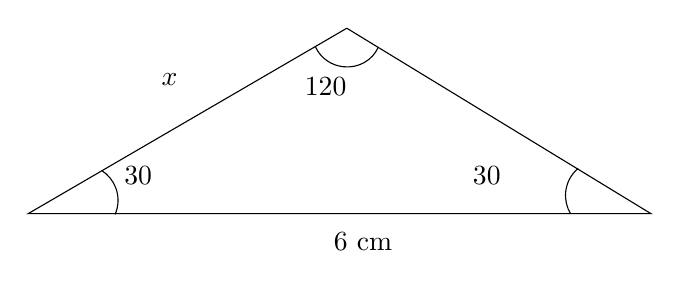
\begin{tikzpicture}[x=0.75pt,y=0.75pt,yscale=-1,xscale=1]
%uncomment if require: \path (0,300); %set diagram left start at 0, and has height of 300

%Shape: Triangle [id:dp9164804627843453] 
\draw   (343.49,20.56) -- (490,109.88) -- (190,109.88) -- cycle ;
%Shape: Arc [id:dp8670513073235429] 
\draw  [draw opacity=0] (358.59,29.81) .. controls (355.84,36.02) and (349.03,39.99) .. (341.63,39.1) .. controls (335.6,38.38) and (330.72,34.63) .. (328.46,29.66) -- (343.49,23.56) -- cycle ; \draw   (358.59,29.81) .. controls (355.84,36.02) and (349.03,39.99) .. (341.63,39.1) .. controls (335.6,38.38) and (330.72,34.63) .. (328.46,29.66) ;  
%Shape: Arc [id:dp6736551053433504] 
\draw  [draw opacity=0] (451.18,109.7) .. controls (449.44,106.76) and (448.58,103.21) .. (448.94,99.48) .. controls (449.4,94.83) and (451.66,90.82) .. (454.92,88.14) -- (464.52,101) -- cycle ; \draw   (451.18,109.7) .. controls (449.44,106.76) and (448.58,103.21) .. (448.94,99.48) .. controls (449.4,94.83) and (451.66,90.82) .. (454.92,88.14) ;  
%Shape: Arc [id:dp020705992733369705] 
\draw  [draw opacity=0] (225.63,89.28) .. controls (228.49,91.15) and (230.83,93.95) .. (232.16,97.45) .. controls (233.81,101.82) and (233.56,106.42) .. (231.83,110.27) -- (217.52,103) -- cycle ; \draw   (225.63,89.28) .. controls (228.49,91.15) and (230.83,93.95) .. (232.16,97.45) .. controls (233.81,101.82) and (233.56,106.42) .. (231.83,110.27) ;  
% Text Node
\draw (235,86) node [anchor=north west][inner sep=0.75pt]   [align=left] {$30 \degree$};
% Text Node
\draw (403,86) node [anchor=north west][inner sep=0.75pt]   [align=left] {$30 \degree$};
% Text Node
\draw (322,43) node [anchor=north west][inner sep=0.75pt]   [align=left] {$120 \degree$};
% Text Node
\draw (253,41) node [anchor=north west][inner sep=0.75pt]   [align=left] {$x$};
% Text Node
\draw (336,118) node [anchor=north west][inner sep=0.75pt]   [align=left] {$6$ cm};
\end{tikzpicture}
\end{center}
     \item  Determine os possíveis valores de $m$ para que exista $x$ em cada caso:
        \begin{enumerate}
            \item   $\sen x = 3m + 8$
            \item   $\cos x = m^2 + m + 1$
        \end{enumerate}
    \item   Dado $\sen x = -\dfrac{2}{3}$, quais são os possíveis valores de $\cos x$ ?
    \item   Calcule o valor do cosseno do ângulo $x$.
\begin{center}     

\begin{tikzpicture}[x=0.75pt,y=0.75pt,yscale=-1,xscale=1]
%uncomment if require: \path (0,300); %set diagram left start at 0, and has height of 300

%Straight Lines [id:da4536831523289997] 
\draw    (292,40) -- (460,180.03) ;
%Straight Lines [id:da2925756071426022] 
\draw    (292,40) -- (210,180.03) ;
%Straight Lines [id:da6307001476948584] 
\draw    (210,180.03) -- (460,180.03) ;
%Shape: Arc [id:dp4868859118866089] 
\draw  [draw opacity=0] (423.47,179.81) .. controls (421.02,173.19) and (423.42,165.14) .. (429.83,160.29) .. controls (431.03,159.37) and (432.3,158.63) .. (433.61,158.05) -- (439.5,173.03) -- cycle ; \draw   (423.47,179.81) .. controls (421.02,173.19) and (423.42,165.14) .. (429.83,160.29) .. controls (431.03,159.37) and (432.3,158.63) .. (433.61,158.05) ;  
%Shape: Arc [id:dp10934028584854505] 
\draw  [draw opacity=0] (222.52,158.37) .. controls (229.18,160.71) and (233.83,167.69) .. (233.48,175.73) .. controls (233.42,177.23) and (233.18,178.69) .. (232.79,180.07) -- (217.5,175.03) -- cycle ; \draw   (222.52,158.37) .. controls (229.18,160.71) and (233.83,167.69) .. (233.48,175.73) .. controls (233.42,177.23) and (233.18,178.69) .. (232.79,180.07) ;  
%Shape: Arc [id:dp4256939613153006] 
\draw  [draw opacity=0] (305.13,51.42) .. controls (300.26,56.53) and (291.98,57.91) .. (284.8,54.29) .. controls (284.3,54.04) and (283.82,53.77) .. (283.35,53.48) -- (292,40) -- cycle ; \draw   (305.13,51.42) .. controls (300.26,56.53) and (291.98,57.91) .. (284.8,54.29) .. controls (284.3,54.04) and (283.82,53.77) .. (283.35,53.48) ;  

% Text Node
\draw (291,57) node [anchor=north west][inner sep=0.75pt]   [align=left] {x};
% Text Node
\draw (228,98) node [anchor=north west][inner sep=0.75pt]   [align=left] {5};
% Text Node
\draw (380,88) node [anchor=north west][inner sep=0.75pt]   [align=left] {6};
% Text Node
\draw (323,186) node [anchor=north west][inner sep=0.75pt]   [align=left] {7};
\end{tikzpicture}
\end{center}


    \item   No retângulo EPCR da figura a seguir, PC = $6$ cm, RA $= 3$ cm e AC $= 5$ cm. 
    \begin{center}
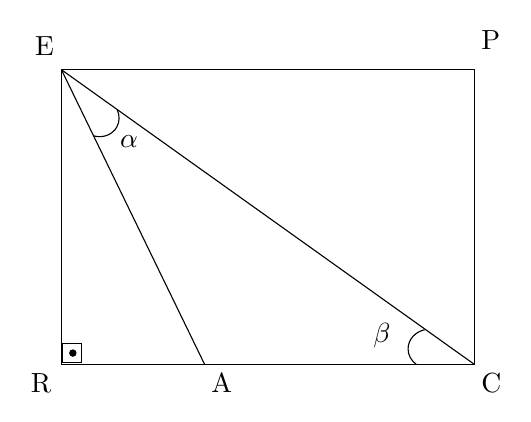
\begin{tikzpicture}[x=0.75pt,y=0.75pt,yscale=-1,xscale=1]
%uncomment if require: \path (0,300); %set diagram left start at 0, and has height of 300

%Shape: Rectangle [id:dp858187982453664] 
\draw   (221,49) -- (420,49) -- (420,191) -- (221,191) -- cycle ;
%Straight Lines [id:da8203153190656269] 
\draw    (221,49) -- (420,191) ;
%Straight Lines [id:da9645069714438275] 
\draw    (221,49) -- (290,191) ;
%Shape: Square [id:dp7139762725461019] 
\draw   (221.25,180.75) -- (230.75,180.75) -- (230.75,190.25) -- (221.25,190.25) -- cycle ;
%Shape: Circle [id:dp6995094064656198] 
\draw  [fill={rgb, 255:red, 0; green, 0; blue, 0 }  ,fill opacity=1 ] (225,185.5) .. controls (225,184.67) and (225.67,184) .. (226.5,184) .. controls (227.33,184) and (228,184.67) .. (228,185.5) .. controls (228,186.33) and (227.33,187) .. (226.5,187) .. controls (225.67,187) and (225,186.33) .. (225,185.5) -- cycle ;
%Shape: Arc [id:dp07469411169597429] 
\draw  [draw opacity=0] (391.89,190.88) .. controls (389.52,189.14) and (388,186.48) .. (388,183.5) .. controls (388,179.04) and (391.4,175.29) .. (395.98,174.27) -- (398.5,183.5) -- cycle ; \draw   (391.89,190.88) .. controls (389.52,189.14) and (388,186.48) .. (388,183.5) .. controls (388,179.04) and (391.4,175.29) .. (395.98,174.27) ;  
%Shape: Arc [id:dp24756523411485687] 
\draw  [draw opacity=0] (247.86,68.26) .. controls (249.09,70.94) and (249.13,74) .. (247.68,76.6) .. controls (245.51,80.5) and (240.72,82.12) .. (236.21,80.79) -- (238.5,71.5) -- cycle ; \draw   (247.86,68.26) .. controls (249.09,70.94) and (249.13,74) .. (247.68,76.6) .. controls (245.51,80.5) and (240.72,82.12) .. (236.21,80.79) ;  

% Text Node
\draw (248,79.58) node [anchor=north west][inner sep=0.75pt]   [align=left] {$\alpha$};
% Text Node
\draw (370,170) node [anchor=north west][inner sep=0.75pt]   [align=left] {$\beta$};
% Text Node
\draw (205,194) node [anchor=north west][inner sep=0.75pt]   [align=left] {R};
% Text Node
\draw (207,32) node [anchor=north west][inner sep=0.75pt]   [align=left] {E};
% Text Node
\draw (422,29) node [anchor=north west][inner sep=0.75pt]   [align=left] {P};
% Text Node
\draw (422,194) node [anchor=north west][inner sep=0.75pt]   [align=left] {C};
% Text Node
\draw (292,194) node [anchor=north west][inner sep=0.75pt]   [align=left] {A};
\end{tikzpicture}
\end{center}

O valor de $\sen \alpha + \cos \alpha$ é

        \begin{enumerate}
            \item   $\dfrac{3\sqrt{5}}{5}$
            \item   $\dfrac{4\sqrt{5}}{5}$
            \item   $\dfrac{2\sqrt{5}}{5}$
            \item   $\dfrac{\sqrt{5}}{5}$
        \end{enumerate}
    \item   Expresse em radianos:
        \begin{enumerate}
            \item $200 \degree$
            \item $9 \degree$
            \item $20 \degree$
            \item $240 \degree$
        \end{enumerate}
    \item   Dê as expressões gerais dos arcos côngruos a:
        \begin{enumerate}
            \item   $2000 \degree$
            \item   $1700 \degree$
        \end{enumerate}
    \item   Calcule as expressões:
        \begin{enumerate}
            \item   $\cos \dfrac{\pi}{3} + \cos \dfrac{\pi}{4} - \cos 2\pi$
            \item   $2 \cos \dfrac{\pi}{6} + \dfrac{1}{2} \cos \dfrac{7\pi}{4}$
            \item   $3 \cos \dfrac{\pi}{2} - 2 \cos \dfrac{5\pi}{4} + \dfrac{1}{2} \cos \pi$
        \end{enumerate}
 \end{enumerate}

 \section{Respostas dos exercícios}

 \begin{enumerate}
    \item $\sen 45 \degree = \dfrac{\sqrt{2}}{2}$; 
     $\cos 45 \degree = \dfrac{\sqrt{2}}{2}$; 
     $\tg 45 \degree = 1$; \\ [0.25cm]
     $\sen 60 \degree = \dfrac{\sqrt{3}}{2}$; 
     $\sen 60 \degree = \dfrac{1}{2}$; 
     $\sen 60 \degree = \sqrt{3}$.     
    \item   Figura \ref{fig:fig05_circtrigcompl} {\color{green!65!black}\faIcon{link}}
    \item   $3\sqrt{3}$cm.
    \item   
        \begin{enumerate}
            \item $-3 < m \le -\dfrac{7}{3}$
            \item $-1 < m \le 0$
        \end{enumerate}
    \item   $\cos x = -\dfrac{\sqrt{5}}{3}$ ou $\cos x = \dfrac{\sqrt{5}}{3}$
    \item   $\cos x = \dfrac{1}{5}$
    \item Alternativa a) $\dfrac{3 \sqrt{5}}{5}$
    \item   
        \begin{enumerate}
            \item $\dfrac{10 \pi}{9}$
            \item $\dfrac{\pi}{20}$
            \item $\dfrac{\pi}{9}$
            \item $\dfrac{4 \pi}{3}$
        \end{enumerate}
    \item
        \begin{enumerate}
            \item $200 \degree + 360 \degree \cdot k, \; k \in \mathbb{Z}$
            \item $260 \degree + 360 \degree \cdot k, \; k \in \mathbb{Z}$
        \end{enumerate}
    \item   
        \begin{enumerate}
            \item $\dfrac{-1 + \sqrt{2}}{2}$
            \item $\sqrt{3} + \dfrac{\sqrt{2}}{4}$
            \item $\sqrt{2} + \dfrac{1}{2}$
        \end{enumerate}
 \end{enumerate}


 